% ###################    CONFIGURACIÓN ################### 

% Configuración de estilos generales de la página
\documentclass[12pt,
               % twocolumn
              ]{article}
              
\usepackage[paperheight=297mm,
			paperwidth=210mm,
			tmargin=28mm, 
			headheight=0mm, 
			headsep=15mm,
			textheight=240mm,
			footskip=7mm,
			textwidth=159.2mm,
			bindingoffset=10mm,
			twoside
			]{geometry} 
% -------------------------------------------------------   


% Configuración de párrafos
% -------------------------------------------------------         
\setlength{\parindent}{0em} % Tabulación de un párrafo nuevo
\setlength{\parskip}{1em}   % Distancia en blanco entre un párrafo y otro.
\setlength{\columnsep}{1em} % Margen izquierdo de columnas
\renewcommand{\baselinestretch}{1.5} % Interlineado. Espacio entre dos renglones.
% ------------------------------------------------------- 


% Paquetes de idioma
\usepackage[utf8]{inputenc}
\usepackage[spanish,english,es-tabla]{babel} % English para el abstract
% ------------------------------------------------------- 

% Paquetes para imprimir código fuente
%\usepackage[cache=false]{minted}

\usepackage{subcaption}

\usepackage[table,xcdraw]{xcolor} % Color de tabla

%\usepackage{movie15}

% Para símbolos de comprobación y x.
\usepackage{pifont}% http://ctan.org/pkg/pifont
\newcommand{\cmark}{ \color{green} \ding{51}}%
\newcommand{\xmark}{ \color{red}\ding{55}}%


% -------------------------------------------------------  

% Paquetes generales
\usepackage{enumitem} % Para configurar enumeraciones
%\usepackage[usenames,dvipsnames]{xcolor}    % Para colores en el texto

% Lorem ipsum
\usepackage[pangram]{blindtext}

\usepackage{scrextend} % Para entorno{addmargin} (dar margen a un párrafo...)

% Lorem ipsum
\usepackage{lipsum}

\usepackage{fancyhdr}

\usepackage{float} % para controlar la situación de los entornos flotantes

\usepackage{graphicx} % figuras

% Definimos un nuevo color
\definecolor{webred}{rgb}{0.5, 0, 0}   % less intense red

\usepackage[bookmarks=true,
			bookmarksnumbered=false, % true means bookmarks in 
									 % left window are numbered                         
			bookmarksopen=false,     % true means only level 1
									 % are displayed.
			colorlinks=true,
			linkcolor=webred,
			%linkcolor=OliveGreen,
			citecolor=webred,
			urlcolor=cyan]{hyperref} % Para hiperenlaces

% Definimos una nueva orden para pintar una línea cuando escribamos \HRule
\newcommand{\HRule}{\rule{\linewidth}{1mm}}




% ###################   FIN CONFIGURACIÓN ################### 

% ###################	INICIO DEL DOCUMENTO ###################

\begin{document}

\thispagestyle{empty}

	\begin{figure}[h]
		\centering
		
\includegraphics[width=0.7\textwidth]{images/logoUGR.jpg}
		\label{imagen2}
	\end{figure}

	\begin{center}
		\Large{TRABAJO FIN DE MÁSTER} \\
		\large{INGENIERÍA INFORMÁTICA}
	\end{center}
	
	\vspace{0.5cm}
	
	\hrule
	
	\begin{center}
		\huge{\textbf{Sistema de videovigilancia con una Raspberry PI}}
	\end{center}
	
	\hrule
	
	\vspace{0.5cm}
	
	\begin{center}
		\textbf{Autor} \\
		Jonathan Martín Valera (alumno)\\
		\textbf{Directores}\\
		Juan Julián Merelo Guervós (tutor)
	\end{center}
	
	\vspace{0.6cm}
	
	\begin{figure}[h]
		\centering
		
\includegraphics[width=0.3\textwidth]{images/etsiit_logo.png}\\[0.1cm]
	\end{figure}
	
	\begin{center}
	\textsc{Escuela Técnica Superior de Ingenierías Informática y de Telecomunicación}\\
	\textsc{---}\\
	Granada, septiembre de 2019
	\end{center}
	
	\newpage

\thispagestyle{empty}

\section*{Agradecimientos}

Después de todo este periodo de formación académica, puedo mirar hacia atrás y hacer una retrospectiva de todo lo sucedido en estos años.

Ha sido una etapa bastante dura e intensiva; una etapa donde se ha tenido que superar grandes obstáculos y emplear muchísima dedicación y esfuerzo. Puedo decir con satisfacción que ha valido la pena. Considero que en esta etapa he adquirido una gran madurez mental, en la que no solo he aprendido algunos conceptos específicos, sino que que puedo decir que he aprendido a pensar y a ser autocrítico con el trabajo.

Gracias al grado y máster de ingeniería informática, veo la realidad de otra forma, con capacidad de poder realizar cualquier reto que me pueda proponer. Si tuviera que resumir en una frase todo lo aprendido en estos años, sería: \textit{`No esperes a que nadie te diga como hacer las cosas, simplemente investiga, experimenta y saca tus propias conclusiones'}.

Este trabajo fin de máster es un ejemplo de ello, una idea hipotética, en la que he investigado, aprendido lo necesario para llevarla a cabo e implementado con éxito.

Quiero agradecer a todos los profesores que he tenido a lo largo de estos años, con especial atención a mi tutor Juan Julián Merelo Guervós, que me ha enseñado en este último año a investigar y conocer una gran cantidad de herramientas actuales que me están siendo de gran utilidad en mi día a día laboral.

Finalmente, agradecer a mis padres la ayuda que, a su forma cada uno, me han proporcionado
en todo este periodo, a mis tíos por apoyarme, motivarme y confiar siempre en mí, y
especialmente a mi novia Nerea, que me ha estado animando todo este tiempo y dando apoyo
moral además de ser fuente de inspiración y superación en mí.

\newpage



\thispagestyle{empty}

\vspace*{\fill} % Para alinear el contenido de la paǵina verticalmente.

\begin{center}
	\textbf{Sistema de videovigilancia con una Raspberry PI}\\
	
	\vspace{0.3cm}
	
	Jonathan Martín Valera (alumno)	\\
	
	\footnotesize{Estudiante de Informática en Escuela Técnica Superior Informática y Telecomunicación, Universidad de Granada, 18071, Granada, España} \\
	
\end{center}

\selectlanguage{spanish}

\begin{abstract}

\noindent \textbf{Palabras clave}: videovigilancia, sistema de seguridad, raspberry PI. 

\vspace{0.2cm}

\noindent Este proyecto se basa en el desarrollo e implementación de un sistema de videovigilancia de bajo coste, haciendo uso de una raspberry PI y sus componentes. La idea es tener una raspberry PI equipada con una cámara y un sensor de movimiento para poder utilizarla como sistema de seguridad, controlada a través de un dispositivo móvil usando la aplicación de Telegram. 

\noindent La aplicación consta de una serie de modos (manual, automático y streaming) con los que se puede vigilar la zona que desees, y enviar alertas automáticas a tu móvil en el caso de detectar alguna actividad sospechosa, capturar imágenes o grabar vídeos de forma manual, o visualizar la retransmisión en directo de la visualización de la cámara, y todo esto se puede controlar desde cualquier localización.

\end{abstract}

\selectlanguage{english} 

\begin{abstract}

\noindent \textbf{Keywords}: video surveillance, security system, raspberry PI.

\vspace{0.2cm}

\noindent This project is based on the development and implementation of a low-cost video surveillance system, using a raspberry PI and its components. The idea is to have a PI raspberry equipped with a camera and a motion sensor to be used as a security system, controlled through a mobile device using the Telegram application. 	

\noindent The application consists of a series of modes (manual, automatic and streaming) with which you can monitor the area you want, and send automatic alerts to your mobile in the event of detecting any suspicious activity, capture images or record videos manually, or view the live broadcast of the camera display, and all this can be controlled from any location.

\end{abstract}

\vspace*{\fill} % Para alinear el contenido de la paǵina verticalmente.

\selectlanguage{spanish}

\newpage


\thispagestyle{empty}


\noindent\rule[-1ex]{\textwidth}{2pt}\\[4.5ex]

Yo, \textbf{Jonathan Martín Valera}, alumno de la titulación máster de ingeniería informática de la \textbf{Escuela Técnica Superior de Ingenierías Informática y de Telecomunicación de la Universidad de Granada}, con DNI 77144272-H, autorizo la ubicación de la siguiente copia de mi Trabajo Fin de Máster en la biblioteca del centro para que pueda ser consultada por las personas que lo deseen.

\vspace{0.5cm}

\noindent Fdo: Jonathan Martín Valera

\begin{figure}[h]
	\centering
	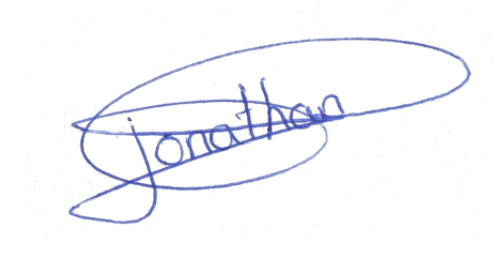
\includegraphics[scale=0.3]{images/firma}
\end{figure}

\begin{flushright}
Granada a 24 de agosto de 2019.
\end{flushright}


\newpage

\thispagestyle{empty}

\noindent\rule[-1ex]{\textwidth}{2pt}\\[4.5ex]

D. Juan Julián Merelo Guervos (tutor), Profesor del Departamento de Arquitectura y Tecnología de Computadores de la Universidad de Granada.

\textbf{Informa:}

Que el presente trabajo, titulado sistema de videovigilancia con una Raspberry PI, ha sido realizado bajo su supervisión por Jonathan Martín Valera (alumno), y autorizamos la defensa de dicho trabajo ante el tribunal que corresponda.

Y para que conste, expiden y firman el presente informe en Granada a 24 de agosto de 2019.


\textbf{El director:}

\begin{figure}[h]
	\centering
	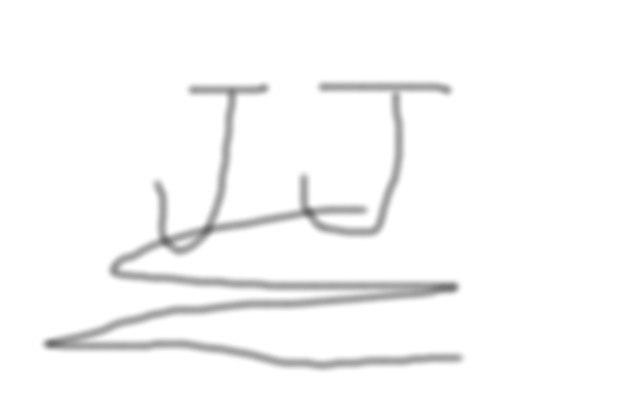
\includegraphics[scale=0.2]{images/firma2}
\end{figure}

\newpage

\fancypagestyle{miEstilo1}{
   \lhead{1. Introducción}
   %\chead{1. Introducción}
   \rhead{Página \thepage}
   \lfoot{}
   \cfoot{}
   \rfoot{}
}

\pagestyle{miEstilo1}

\section{Introducción}

\subsection{Motivación}

El número de robos y hurtos ha ido creciendo en estos últimos años, y por ello, es necesario la aplicación de medidas preventivas y correctoras que intenten reducir este número.

Hoy en día vivimos en una sociedad informatizada y tecnológica, donde cada uno tiene la capacidad de poder encontrar casi cualquier información allá donde esté, gracias a los dispositivos móviles y a la redes de comunicaciones que usa internet.

¿Quién no lleva un smartphone con conexión de datos en su bolsillo? En España el 85\% de la población hace uso de su smartphone a diario. Estos dispositivos móviles tienen una gran cantidad de usos y aplicaciones, y se han convertido en una herramienta imprescindible en nuestro día a día.

Uniendo tecnología y aplicación de medidas de seguridad basada en videovigilancia, surge la idea de este proyecto; la idea de construir un sistema de videovigilancia de bajo coste que sea fácil de usar, mantener, y lo más importante, que pueda ser controlado desde cualquier parte.

Partiendo de esta idea, se ha investigado y construido una aplicación que cumple con estas expectativas y más, ya que el uso que se le quiera dar puede ir más allá del concepto de videovigilancia para la seguridad. Por ejemplo, se puede utilizar para controlar entradas y salidas en una zona, control parental \ldots, aunque eso sí, dentro de un uso permitido y responsable.

Otro de los principales aspectos de este proyecto, es que su uso no sea de forma privada, es decir, que pueda ser usado por todas las personas que lo deseen. Por este motivo, se ha intentado reducir todo lo posible el coste del hardware, y se ha liberado todo el código fuente, junto con las instrucciones necesarias para la instalación y despliegue de la aplicación.

Toda la información relacionada se puede consultar en el repositorio de Github \cite{ref1}.

\subsection{Objetivos}

El objetivo principal de este proyecto es el de poder construir un sistema de seguridad basado en la videovigilancia, de bajo coste, y accesible a todo el mundo.

\textbf{Objetivos generales}

\vspace{-0.3cm}

\begin{itemize}
	\item Rebajar el coste de los sistemas de videovigilancia habituales.
	\item Alertar a un usuario ante un evento de movimiento generado dentro de una zona controlada.
	\item Almacenar y obtener pruebas (fotos y/o vídeo) tras la detección de cualquier intruso.
	\item Monitorizar y controlar el estado de un entorno.
	\item Aumentar el nivel de seguridad de cualquier tipo de entorno.	
\end{itemize}

\textbf{Objetivos específicos}

\vspace{-0.3cm}

\begin{itemize}
	\item Proporcionar un sistema accesible para todo el mundo y fácil de usar.
	\item Permitir el acceso y gestión del sistema a través de un dispositivo móvil.
	\item Investigar y conocer el uso de los bots de Telegram como medio de interacción entre el usuario y la aplicación back-end desarrollada en este proyecto.
	\item Estudiar el funcionamiento de una Raspberry PI y sus principales componentes para su aplicación en el ámbito del proyecto.
	\item Conocer, diseñar y hacer uso de una arquitectura basada en microservicios que permita el uso de servicios independientes, ágiles y escalables.
	\item Aprender a utilizar mecanismos de aprendizaje automático para poder filtrar y evitar falsos positivos en las alertas generadas.

\end{itemize}

\newpage

\subsection{Estructura del documento}

Este documento está estructurado de la siguiente forma:

\textbf{1. Introducción}: Motivos y objetivos por los cuales se ha desarrollado este proyecto.

\textbf{2. Planificación del proyecto}: Muestra información detallada acerca de las diferentes etapas del proyecto, junto con la planificación prevista.

\textbf{3. Análisis de mercado}: Estudio comparativo acerca de softwares similares al propuesto en este proyecto.

\textbf{4. Tecnologías y herramientas utilizadas}: Breve descripción sobre las tecnologías y herramientas utilizadas para desarrollar este proyecto.

\textbf{5. Descripción de la aplicación: SIVIRA}: Descripción sobre los componentes de la aplicación, la interacción entre ellos, medidas de seguridad aplicadas, interfaz de usuario y descripción de la estructura de archivos y directorios de la aplicación.

\textbf{6. Presupuesto}: Estimación de costes del desarrollo del proyecto junto con una previsión de futuros beneficios en el mercado laboral.

\textbf{7. Conclusiones y trabajos futuros}: Conclusiones tras finalizar el desarrollo del proyecto y posibles mejoras a desarrollar en versiones posteriores.

\textbf{ANEXO}: Información útil sobre la aplicación SIVIRA: guía de instalaciones de componentes, instalación y despliegue de la aplicación y finalmente una guía de usuario.

\newpage



\newpage



\fancypagestyle{miEstilo2}{
   \lhead{2. Planificación}
   %\chead{1. Introducción}
   \rhead{Página \thepage}
   \lfoot{}
   \cfoot{}
   \rfoot{}
}

\pagestyle{miEstilo2}

\section{Planificación}

Como en todo proyecto, realizar una buena planificación es la clave para no fracasar en el desarrollo del proyecto. Por ello, se ha realizado una planificación detallada del proyecto, utilizando el concepto de \textit{iteraciones} y \textit{sprints} para ir distribuyendo el trabajo a lo largo de las semanas, durante las cuales se han ido desarrollando una serie de tareas que cumplen un objetivo específico.

Estos conceptos surgen de los llamados métodos de desarrollo ágiles, en los cuales se intenta descomponer una aplicación o proyecto por funcionalidades, y el objetivo es ir desarrollando y testeando cada una de forma independientes para poder integrarla con el resto.

A continuación se muestra la planificación que se ha previsto para el desarrollo del proyecto.


\subsection{Fase preparatoria}

En esta fase se comenzará el desarrollo del proyecto. Tiene un esfuerzo estimado de X horas. Se realizará un estudio de viabilidad de la idea del proyecto, así como un estudio de mercado, una investigación acerca de las posibles herramientas a usar \ldots.

El objetivo de esta primera fase es tener claro que el proyecto es viable tanto en recursos, tiempo y presupuesto, para que posteriormente comience su desarrollo e implementación.

\large{\textbf{Iteración 1}: Análisis y estudio de la aplicación.}
\hrule

\vspace{0.3cm}

\normalsize

En esta iteración se describirán los principales objetivos de la aplicación, se estudiará sus posibles casos de uso y se elaborará un plan de iteraciones para planificar el desarrollo del proyecto a lo largo del tiempo dispuesto.

Esta iteración se divide en los siguientes sprints:

\textbf{Sprint 1}: Descripción de la aplicación



%\begin{center}
%\begin{tabular}{ | m{5em} | m{1cm}| m{1cm} | } 
%\hline
%cell1 dummy text dummy text dummy text& cell2 & cell3 \\ 
%\hline
%cell1 dummy text dummy text dummy text & cell5 & cell6 \\ 
%\hline
%cell7 & cell8 & cell9 \\ 
%\hline
%\end{tabular}
%\end{center}




\begin{table}[]
\begin{tabular}{|p{4cm}|p{7cm}|p{1.5cm}|p{2.5cm}|}
\hline
\rowcolor[HTML]{000000} 
{\color[HTML]{FFFFFF} Product backlog} & {\color[HTML]{FFFFFF} Descripción}                                  & {\color[HTML]{FFFFFF} Semana} & {\color[HTML]{FFFFFF} T.Previsión} \\ \hline
Objetivos                              & Descripción de los objetivos                                        & 1                             &                                        \\ \hline
Funcionalidades                        & Descripción de las funcionalidades                                  & 1                             &                                        \\ \hline
Motivaciones                           & Motivaciones personales acerca de la temática del proyecto          & 1                             &                                        \\ \hline
Usuarios y escenarios                  & Descripción de los posibles casos de uso de la aplicación propuesta & 1                             &                                        \\ \hline
\end{tabular}
\end{table}






\newpage



\fancypagestyle{miEstilo3}{
   \lhead{3. Análisis de mercado}
   %\chead{1. Introducción}
   \rhead{Página \thepage}
   \lfoot{}
   \cfoot{}
   \rfoot{}
}

\pagestyle{miEstilo3}

\section{Análisis de mercado}

Antes de comenzar con el desarrollo del proyecto, se ha realizado un estudio de mercado para comprobar si hay algún tipo de sistema similar ya implementado, qué características tiene, y qué posibles diferencias habría con el que se tiene pensado implementar.

Es cierto que la raspberry PI tiene infinidades de posibles aplicaciones, y que en la web se puede encontrar todo tipo de tutoriales e ideas para poder explotar al máximo su uso, pero ¿existirá algún tipo sistema de seguridad que sea funcional, fácil de instalar y utilizar?. Para responder a esta pregunta, se ha realizado una búsqueda intensiva en la web y youtube, ya que suelen ser los principales medios donde se publica este tipo de información.

Investigando, se ha descubierto que hay múltiples páginas y vídeos que hacen referencia al uso de una raspberry PI con una cámara, y su posible aplicación para poder visualizar en tiempo real la grabación realizada por la cámara.

A continuación se van a detallar los principales aspectos a destacar de los sistemas encontrados.

\subsection{Proyecto: Build a Raspberry Pi Security Camera Network} \label{sec:pj1}

Este es un proyecto \cite{ref2} que se basa en el uso de una distribución Linux llamada \texttt{motionEyeOS} y de código abierto \cite{ref3} que convierte una raspberry PI en un sistema de videovigilancia.

Si leemos la descripción de este proyecto \cite{ref2}, podemos observar como se hace una pequeña descripción de los componentes necesarios y una guía de instalación del sistema \texttt{motionEyeOS}.

Entre sus principales características, podemos encontrar las siguientes:

\vspace{-0.5cm}

\begin{itemize}
\item \textbf{Acceso restringido}: Consta de unas credenciales (usuario y contraseña) para poder acceder a la visualización y configuración de las cámaras.

\item \textbf{Sistema multicámara}: Es un sistema que soporta la visualización e interacción con múltiples cámaras simultáneamente conectadas en la misma red.

\begin{figure}[h]
	\centering
	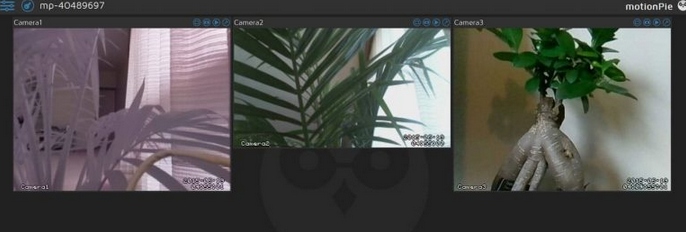
\includegraphics[scale=0.4]{images/1}
	\label{imagen2}
	\caption{Sistema de seguridad con 3 cámaras}
\end{figure}

\item \textbf{Conexión via wifi}: Este sistema soporta la conexión via wifi. Será necesario añadir el SSID y clave de la red.

\item \textbf{Configuración de la cámara}: El sistema consta de un menú para poder configurar la cámara. Los parámetros configurables son:

	\begin{itemize}
	\item Nombre de la cámara: Nombre para poder identificar la cámara.
	\item Filtrado de luz: Filtro para evitar falsos positivos ante el encendido y apagado de una luz.
	\item Brillo automático: Configuración automática de brillo y contraste de luz.
	\item Resolución de la cámara: Configuración para poder modificar la resolución de la cámara.
	\item Rotación de la cámara: Rotación de la imagen de vídeo o cámara.
	\item FPS: Configuración del número de frames por segundo (imágenes por segundo).
	\end{itemize}

\item \textbf{Almacenamiento}: Es posible almacenar los archivos de imagen o vídeo.

\item \textbf{Fecha y hora}: Posibilita la opción de mostrar fecha y hora durente la grabación de un vídeo o la captura de una foto.

\item \textbf{Vídeo streaming}: Permite la visualización del vídeo capturada por las cámaras en tiempo real.

\item \textbf{Detección de movimiento}: El sistema permite la detección de movimiento y en consecuencia la grabación de un vídeo o la captura de una foto.

\item \textbf{Alertas}: Es posible generar alertas via email o webhook cuando se detecta movimiento.

\end{itemize}

\subsection{Proyecto: Raspberry Pi As Low-cost HD Surveillance Camera}\label{sec:pj2}

Este es un proyecto \cite{ref4} bastante simple y centrado en la vigilancia y basado en \texttt{Motion detection software} \cite{ref5}. Este es un software de código abierto y disponible en los repositorios de raspbian para poder monitorizar las señales de vídeo para varios tipos de cámaras (entre ellas la PiCamera).

Algunas de las características de este software son:

\vspace{-0.5cm}

\begin{itemize}
\item Grabación de vídeos y/o capturas de fotos.
\item Visualización de vídeo en tiempo real (streaming).
\item Gestión de actividades y activación de scripts tras dichos eventos.
\item Registro de eventos en bases de datos.
\item Plantillas personalizables para detección de movimiento.
\item Soporte completo de TLS (https) con autenticación y control web para streaming.

\end{itemize}

En este proyecto, se hace una descripción de los componentes necesarios para poder montar este sistema, e incluso se hace una estimación del precio de dichos componentes y se proporciona un enlace de compra.

A continuación se proporciona una guía básica de instalación y configuración, mostrando los siguientes resultados:

\newpage

\begin{figure}[H]
	\centering
	\begin{subfigure}[b]{0.3\textwidth}
		
\includegraphics[width=\textwidth,height=90px]{images/2}
		\caption{Colocación de la cámara}
	\end{subfigure}
	~ 
	\begin{subfigure}[b]{0.3\textwidth}
		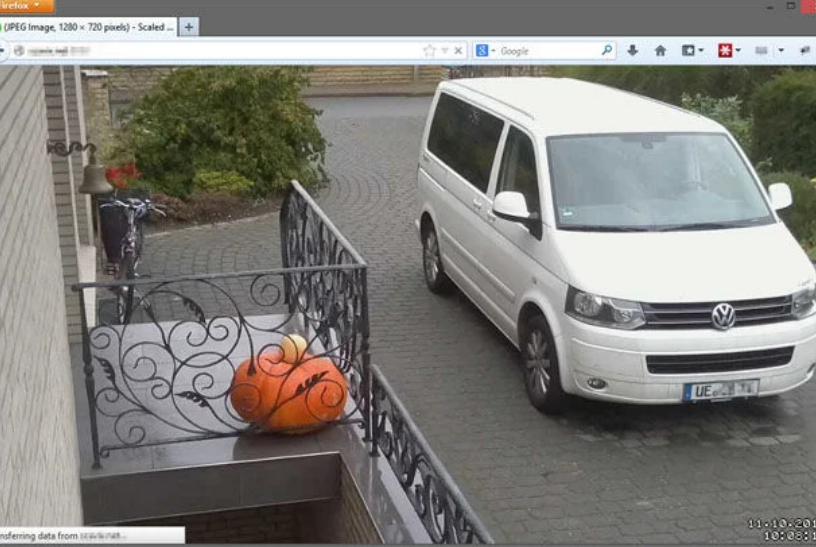
\includegraphics[width=\textwidth,height=90px]{images/3}
		\caption{Streaming}
	\end{subfigure}
	\caption{Sistema de videovigilancia}

\end{figure}

\subsection{Proyecto: sensor de movimiento y cámara con envío de imágenes a correo} \label{sec:pj3}

Este es un proyecto descrito en un vídeo de youtube \cite{ref6} que explica cómo construir un pequeño sistema de seguridad basado en la detección de movimiento, captura de una foto y envío de la foto capturada tras haberse activado la detección de movimiento.

En este vídeo se explica qué componentes son necesarios, cómo conectarlos y se proporciona un script de Python que se encarga de la detección movimiento y envío de la imagen al correo gmail, utilizando librerías de Python como \textit{PiCamera} y \textit{smtplib}.

Este proyecto no tiene complejidad alguna, ya que es muy simple y todo está explicado para cualquier usuario, y es un buen comienzo para empezar a investigar y probar el mundo de la videovigilancia basada en bajo coste.

\subsection{Conclusión}

Investigando por la web, he descubierto que hay muchos tipos de proyectos similares a los mencionados, unos más simples y otros más complejos, pero en general todos comparten el objetivo de poder vigilar una zona a través de una cámara y una raspberry PI.

\newpage

Otro de los principales aspectos a destacar, es que la mayoría hacen el uso del software libre \texttt{motionEyeOS} o \texttt{motion agent detection} que se han mencionado en las secciones \ref{sec:pj1} y \ref{sec:pj2}.

El objetivo de este proyecto no es 'volver a reinventar la rueda` sino hacer de este un proyecto innovador y con un valor añadido respecto al resto.

Por ello, se ha diseñado y propuesto un sistema que cumpla con la mayoría de características de proyectos similares, combinando lo mejor de cada uno, y añadiendo nuevas funcionalidades adicionales que hagan que sea una de las mejores opciones a la hora de plantearse implementar un sistema de videovigilancia de bajo coste.

Según he podido observar, hay muchos proyectos en los que la documentación es escasa y no muy concisa, además de realizar instalaciones y configuraciones a bajo nivel. Esto hace que cualquier usuario no tenga acceso a este tipo de aplicaciones, ya que requieren un usuario medio-avanzado en conocimientos informáticos.

Por ello, se ha tenido en cuenta la simplicidad del software y su fácil gestión y uso, además de intentar cubrir todos los principales aspectos de una videovigilancia.

En las siguientes secciones, se mostrará más en detalle qué funcionalidades tiene esta aplicación, pero para mostrar sus principales aspectos clave y diferenciadores respecto al resto se va a realizar una comparación, tal y como se puede observar en la siguiente tabla.


Observando la tabla \ref{table:1}, se puede comprobar como la aplicación propuesta cumple con la mayoría de las características del resto de proyectos actuales, y mejora en otros aspectos.

Como aspecto a destacar, decir que el proyecto propuesto consta de una aplicación backend y una aplicación multiplataforma de usuario, además de ser fácil de usar y estar documentada. Estos aspectos principales aportan una gran versatilidad a este proyecto, siendo sin duda la mejor opción hasta el momento desarrollada en el ámbito de la videovigilancia de raspberry PI.

También, como trabajos futuros, se desea implementar la funcionalidad multicámara, haciendo posible la interacción con más de una cámara simultáneamente.

\newpage

\begin{table}[h!]
\centering
\begin{tabular}{|l|c|c|c|c|}
\hline
\rowcolor[HTML]{EFEFEF} 
 \textbf{ Proyectos} & \hyperref[sec:pj1]{Proyecto 1}  & \hyperref[sec:pj2]{Proyecto 2} & \hyperref[sec:pj3]{Proyecto 3} & Mi propuesta \\ \hline
Captura de imagen & \cmark & \cmark  & \cmark & \cmark \\ \hline
\rowcolor[HTML]{fcfcfc} 
Grabación de vídeo & \cmark  & \cmark  & \xmark & \cmark \\ \hline
Streaming & \cmark  & \cmark & \xmark & \cmark \\ \hline
\rowcolor[HTML]{fcfcfc} 
Alertas & \cmark  & \cmark & \cmark & \cmark \\ \hline
Filtrado de alertas inteligente & \xmark   & \xmark & \xmark & \cmark \\ \hline
\rowcolor[HTML]{fcfcfc} 
Aplicación de usuario & \xmark & \xmark & \xmark & \cmark \\ \hline
Soporte multicámara & \cmark  & \cmark & \xmark & \xmark \\ \hline
\rowcolor[HTML]{fcfcfc} 
Fácil instalación y uso & \xmark  & \xmark & \cmark & \cmark \\ \hline
Cámara configurable & \cmark  & \xmark & \xmark & \cmark \\ \hline
\rowcolor[HTML]{fcfcfc} 
Documentación & \xmark & \xmark & \xmark & \cmark \\ \hline
Almacenamiento de eventos & \xmark  & \cmark & \xmark & \cmark \\ \hline
\end{tabular}
\caption{Comparativa de los distintos proyecto}
\label{table:1}
\end{table}

\color{black}


\newpage



\fancypagestyle{miEstilo4}{
   \lhead{4. Tecnologías y herramientas usadas}
   %\chead{1. Introducción}
   \rhead{Página \thepage}
   \lfoot{}
   \cfoot{}
   \rfoot{}
}

\pagestyle{miEstilo4}

\section{Tecnologías y herramientas utilizadas}

Para el desarrollo de este proyecto se han utilizado una gran cantidad de herramientas y tecnologías de código abierto. A continuación se muestra cada una de ellas.

\subsection{Diseño}

Para el diseño de este proyecto, se han realizado prototipos y diagramas para poder diseñar la arquitectura y principales componentes de la aplicación, además de la interacción de los componentes con el resto. Para realizar esto, se ha utilizado el siguiente software:

\textbf{Draw.io}

Draw.io \cite{ref7} es una aplicación para diseño y diagramas de aplicaciones. Es un servicio gratis de Google y de código abierto.

Este software se ha utilizado para diagramas de diseño de interfaz.

\begin{figure}[h]
	\centering
	
\includegraphics[scale=0.5]{images/4}
\end{figure}

\textbf{Visual paradigm} 

Visual paradigm \cite{ref8}  es un software de modelado UML que nos permite analizar, diseñar,
codificar, probar y desplegar. Dibuja todo tipo de diagramas UML, genera código fuente a
partir de dichos diagramas y también posibilita la elaboración de documentos.


\begin{figure}[h]
	\centering
	
\includegraphics[scale=0.5]{images/5}
\end{figure}

Este software se ha utilizado para la generación del diagrama de clases e interacción entre componentes.

\newpage

\subsection{Sistema control de versiones}

Los sistemas de control de versiones \cite{ref9} son programas que tienen como objetivo controlar los cambios en el desarrollo de cualquier tipo de software, permitiendo conocer el estado actual de un proyecto, los cambios que se le han realizado a cualquiera de sus piezas, las personas que intervinieron en ellos \ldots

El control de versiones es una de las tareas fundamentales para la administración de un proyecto de desarrollo de software en general. Surge de la necesidad de mantener y llevar control del código que vamos programando, conservando sus distintos estados. Es absolutamente necesario para el trabajo en equipo, pero resulta útil incluso a desarrolladores independientes. 

Por este motivo, no he dudado en utilizar un sistema de control de versiones. El sistema de control de versiones me ha facilitado mucho la gestión y seguimiento del proyecto. El sitema que he utilizado ha sido \texttt{git}, y como medio de alojamiento para este proyecto he utilizado  \texttt{Github}.

\textbf{Git}

\texttt{Git} \cite{ref10}  es un sistema de control de versiones distribuido, de código libre y multiplataforma que permite la gestión de repositorios software a través de una línea de comandos \cite{ref9}.

Para este proyecto, se ha creado un repositorio donde se ha almacenado todo el código fuente de la aplicación junto con sus cambios a lo largo de su desarrollo.

\begin{figure}[h]
	\centering
	
\includegraphics[scale=0.25]{images/6}
\end{figure}

\textbf{Github}

\texttt{Github} \cite{ref11} es un servicio para alojamiento de repositorios de software gestionados por el sistema de control de versiones \texttt{Git}. En definitiva, \texttt{Github} es un sitio web pensado para hacer posible el compartir el código de una manera más fácil y al mismo tiempo darle popularidad a la herramienta de control de versiones en sí, que es \texttt{Git}.

Este proyecto se ha ido alojando en el repositorio de Github \url{https://github.com/jmv74211/TFM_security_system_PI}.

\begin{figure}[h]
	\centering
	
\includegraphics[scale=0.2]{images/7}
\end{figure}

\subsection{Lenguajes de programación y lenguajes de marcas}

La implementación de este proyecto está desarrollada básicamente en \texttt{Python}. También se ha hecho uso de otros lenguajes de programación para alguna tarea en particular.

A continuación se muestran los lenguajes de programación utilizados.

\textbf{Python}

\texttt{Python} es un lenguaje de programación interpretado, de alto nivel y de propósito general. Este lenguaje de programación viene instalado predeterminadamente en casi todos los sistemas operativos, y consta de un gran número de bibliotecas para realizar una gran cantidad de tareas.

\texttt{Python} se ha utilizado como lenguaje de programación base, con aproximadamente un 90\% del código fuente total. Básicamente he elegido este lenguaje ya que Raspberry PI posee bibliotecas para interaccionar con \texttt{Python}, y con el resto de componentes involucrados.

\begin{figure}[h]
	\centering
	
\includegraphics[scale=0.13]{images/8}
\end{figure}

\textbf{HTML, CSS y Javascript}

Para poder visualizar el streaming de vídeo a través del navegador, ha sido necesario implementar una pequeña página web utilizando \texttt{HTML} y \texttt{CSS}. Respecto a la parte de conexión entre la cámara y el navegador se ha utilizado \texttt{Python} para crear el servidor HTTP y la conexión websocket, y una biblioteca de funciones de \texttt{Javascript} para la transmisión de datos.

\vspace{-0.5cm}

\begin{figure}[h]
	\centering
	
\includegraphics[scale=0.7]{images/9}
\end{figure}

\vspace{-1cm}

\textbf{BASH}

Bash es un intérprete de comandos que ejecuta, una por una, las instrucciones introducidas por el usuario o contenidas en un script y devuelve los resultados. En otras palabras, actúa como interfaz entre el kernel Linux y los usuarios o programas del modo texto. Además, incorpora numerosas utilidades de programación y mejoras sobre sh, su shell predecesora. Debido a que es una herramienta desarrollada por GNU, suele ser utilizada por defecto en las distros actuales.

\begin{figure}[h]
	\centering
	
\includegraphics[scale=0.15]{images/10}
\end{figure}

En este proyecto se ha programado un script en \texttt{bash} para iniciar o parar la aplicación.

\subsection{Bibliotecas y frameworks externos}

Para la implementación de este proyecto, se han utilizado un gran número de bibliotecas para poder interaccionar entre sus distintos componentes.

A continuación se describen brevemente las bibliotecas y frameworks utilizados.

\newpage

\textbf{PiCamera}

\texttt{PiCamera} \cite{ref12} es una biblioteca de \texttt{Python} que proporciona una gran cantidad de funciones para interaccionar directamente con la cámara de la Raspberry PI.

Esta biblioteca ha sido utilizada en los módulos que interactúan directamente con el recurso hardware de la cámara.


\begin{figure}[h]
	\centering
	
\includegraphics[scale=0.09]{images/11}
\end{figure}

\textbf{pyTelegramBotAPI}

\texttt{pyTelegramBotAPI} \cite{ref13} es una biblioteca de funciones de alto nivel que hace uso de la API de Telegram.

En este proyecto se ha utilizado para crear el bot de Telegram, que será la aplicación con la que el usuario interaccionará, y éste a su vez con la API desarrollada en la aplicación backend.

\begin{figure}[h]
	\centering
	
\includegraphics[scale=0.22]{images/12}
\end{figure}

\textbf{Flask}

\texttt{Flask} \cite{ref14} es un framework ligero de aplicaciones web WSGI. Está diseñado para hacer que el despliegue de una aplicación sea rápida y fácil, con la capacidad de escalar a aplicaciones complejas.

En este proyecto se ha utilizado para implementar varios servicios web, como la API principal que interactúa con el resto de módulos y componentes.

\begin{figure}[h]
	\centering
	
\includegraphics[scale=0.19]{images/13}
\end{figure}

\textbf{Celery}

\texttt{Celery} \cite{ref15} es una implementación de una cola de tareas para aplicaciones web de \texttt{Python} que se utiliza para ejecutar tareas de forma asíncrona.

En este proyecto se ha utilizado principalmente en la API y en el agente de movimiento. El objetivo es poder realizar peticiones, y que la API atienda al mayor número de ellas, devolviendo la respuesta tras la ejecución de las tareas, sin producir ningún tipo de espera entre las comunicaciones (Más información en la sección \ref{sec:composer}).

\vspace{-0.6cm}

\begin{figure}[h]
	\centering
	
\includegraphics[scale=0.15]{images/14}
\end{figure}

\vspace{-1.4cm}

\textbf{RPi.GPIO}

\texttt{RPi.GPIO} \cite{ref16} es un paquete que provee de una clase para controlar las conexiones GPIO de la Raspberry PI.

En este proyecto es usado para recibir la señal del sensor de movimiento, de forma que es posible saber cuándo se ha activado.

\begin{figure}[h]
	\centering
	
\includegraphics[scale=0.15]{images/15}
\end{figure}

\vspace{-0.6cm}

\textbf{Tensorflow}

\texttt{Tensorflow}  es una plataforma de código abierto para aprendizaje automático. Cuenta con un ecosistema completo y flexible de herramientas, bibliotecas y recursos que permiten a los investigadores impulsar el estado del arte en machine learning y a los desarrolladores construir y desplegar fácilmente aplicaciones potenciadas por el machine learning.

En este proyecto se ha utilizado para construir un agente que sea capaz de reconocer objetos en una foto utilizando un modelo ligero preentrenado (más información en la sección \ref{sec:composer}).

\begin{figure}[h]
	\centering
	
\includegraphics[scale=0.12]{images/19}
\end{figure}

\textbf{Requests}

\texttt{Requests} \cite{ref18} es una librería HTTP con licencia Apache2, escrita en \texttt{Python}. Permite enviar peticiones HTTP/1.1, además de añadir cabeceras, datos de formulario, archivos y parámetros con diccionarios \texttt{Python} simples, y acceder a los datos de respuesta de la misma manera.

En este proyecto ha sido utilizado para la comunicación entre los servicios a través de sus API's.

\begin{figure}[h]
	\centering
	
\includegraphics[scale=0.08]{images/20}
\end{figure}

\vspace{-0.5cm}

\subsection{Documentación}

\textbf{LaTeX}

Para elaborar la documentación se ha utilizado \texttt{LaTeX} \cite{ref19} que es un sistema de elaboración de documentos para una composición tipográfica de alta calidad. Se utiliza con mayor frecuencia para documentos técnicos o científicos de mediano a gran tamaño, pero se puede utilizar para casi cualquier forma de publicación.

Para este proyecto se ha utilizado \texttt{LaTeX}, utilizando la distribución \texttt{TEXLive} \cite{ref20} que proporciona un sistema TeX completo con binarios para la mayoría de las versiones de Unix, incluyendo GNU/Linux, macOS, y también Windows. Incluye todos los principales programas relacionados con TeX, paquetes de macros y fuentes que son software libre, incluyendo soporte para muchos idiomas en todo el mundo. 

\begin{figure}[h]
	\centering
	
\includegraphics[scale=0.18]{images/16}
\end{figure}

\textbf{TeXstudio}

\texttt{TeXstudio} \cite{ref21} es un entorno integrado para crear documentos LaTeX. El objetivo es conseguir que escribir LaTeX sea lo más fácil y cómodo posible.

Para este proyecto se ha utilizado la versión \textit{2.12.14}.

\begin{figure}[h]
	\centering
	
\includegraphics[scale=0.3]{images/17}
\end{figure}

\subsection{Entorno de desarrollo}

El entorno de desarrollo ha sido un aspecto muy importante para la implementación del proyecto, ya que el código se está ejecutando en una Raspberry PI que tiene recursos muy limitados, y los editores o entornos que puede utilizar no son los más cómodos.

Por este motivo, he estado investigando si se puede realizar un desarrollo de la aplicación vía remota. Leyendo foros, observé que el entorno de desarrollo \texttt{pycharm} tiene la opción de poder crear y desarrollar un proyecto vía SSH.

\textbf{Pycharm}

Pycharm \cite{ref22} es un entorno de desarrollo profesional de \texttt{Python}. Gracias a dicho entorno de desarrollo he podido gestionar el proyecto de forma local, ya que los cambios generados se han sincronizado y ejecutado en la Raspberry PI a través de SSH.

En este proyecto se ha utilizado la versión \textit{2019.1.3 Profesional edition}, licencia académica que he obtenido gracias a la UGR. 

\begin{figure}[h]
	\centering
	
\includegraphics[scale=0.06]{images/18}
\end{figure}


\subsection{Otros servicios}

\textbf{Rabbit MQ} 

\texttt{RabbitMQ} \cite{ref23} es un broker de mensajes que acepta y reenvía mensajes. Un broker de mensajes actúa como plataforma intermediaria a la hora de procesar la comunicación entre dos aplicaciones.

En este proyecto ha sido utilizado para crear dos colas de procesos, utilizados por las tareas asíncronas desarrolladas con \texttt{celery}.

\begin{figure}[h]
	\centering
	
\includegraphics[scale=0.2]{images/21}
\end{figure}

\textbf{Telegram bot API} 

Los bots de Telegram \cite{ref24} son aplicaciones de terceros que se ejecutan dentro de Telegram. Los usuarios pueden interactuar con los bots enviándoles mensajes, comandos y peticiones. Se pueden controlar estos bots usando peticiones HTTPS a la API de bot de Telegram.

En este proyecto se ha utilizado para crear un bot de Telegram que interactúe con el usuario y con la aplicación backend desarrollada.

\begin{figure}[h]
	\centering
	
\includegraphics[scale=0.1]{images/22}
\end{figure}




\newpage



\fancypagestyle{miEstilo5}{
   \lhead{5. Descripción de la aplicación}
   %\chead{1. Introducción}
   \rhead{Página \thepage}
   \lfoot{}
   \cfoot{}
   \rfoot{}
}

\pagestyle{miEstilo5}

\section{Descripción de la aplicación: SIVIRA}

El sistema de videovigilancia con una Raspberry PI (\texttt{SIVIRA}) es una aplicación que nos permite construir un sistema de seguridad basado en la videovigilancia de bajo coste utilizando una Raspberry PI , una cámara y un sensor de movimiento.

La idea es poder controlar el sistema a través de una aplicación móvil, con la que el usuario pueda conectarse desde cualquier parte y tener acceso a su información y sistema de seguridad. Las funciones principales de este sistema son las siguientes:

\begin{itemize}
\item \textbf{Sistema automático} de alertas generadas al capturar el movimiento.
\item \textbf{Sistema manual} para grabar vídeo o capturar una foto instantáneamente.   
\item \textbf{Sistema de streaming} para visualizar la imagen en tiempo real.
\end{itemize}

Además, podemos realizar configuraciones personalizadas a la cámara, como por ejemplo, cambiar la resolución, rotación... y la opción de poder activar un agente que filtre las alertas automáticas, generando únicamente alertas cuando se detecta a una persona en una imagen (evitar falsos positivos).

\subsection{Arquitectura de la aplicación}

Esta aplicación consta de una \textbf{arquitectura basada en microservicios}. Una arquitectura de microservicios \cite{ref25} consta de una colección de servicios autónomos y pequeños. Los servicios son independientes entre sí y cada uno debe implementar una funcionalidad de negocio individual.

En cierto modo, los microservicios son la evolución natural de las arquitecturas orientadas a servicios aunque con ciertas diferencias.

\newpage

\textbf{¿Por qué se ha utilizado esta arquitectura?}

En primer lugar, se ha realizado una descomposición de los principales componentes necesarios para construir la aplicación, y se ha observado que hay funcionalidades independientes que se pueden comunicar entre sí para integrarse en la aplicación. Esto aporta una gran serie de ventajas respecto a un diseño monolítico \cite{ref26} como las siguientes:

\begin{itemize}
\item \textbf{Implementaciones independientes}: Es posible actualizar un servicio sin volver a implementar toda la aplicación y revertir o poner al día una actualización si algo va mal. Las correcciones de errores y las publicaciones de características son más fáciles de administrar y entrañan menos riesgo, por lo tanto, facilitan el mantenimiento de este software.

\item \textbf{Desarrollo independiente}: Cada microservicio se ha ido desarrollando a lo largo de una iteración y de forma independiente al resto. Esto ha agilizado bastante la tarea, ya que las modificaciones y errores no se retropropagaban.

\item \textbf{Fácil escalabilidad}: Cada microservicio puede ser escalado de forma independiente al resto. Por ejemplo, en el caso de que sea necesario escalar la detección de objetos en imágenes, bastaría con replicar el microservicio de detección de objetos y balancear las peticiones entre ellos.

\item \textbf{Fácil integración y alta cohesión}: Un sistema de microservicios se puede integrar y adaptar a casi cualquier sistema. Por ejemplo, en el caso de que quisiera añadir un sistema multicámara a la aplicación, bastaría con añadir una nueva capa superior de abstracción sobre el software desarrollado y se integraría perfectamente.
\end{itemize}

Basándome en esta arquitectura basada en microservicios, se ha diseñado el siguiente sistema (ver figura \ref{img:arquitectura}).

\newpage

\begin{figure}[h]
	\centering
	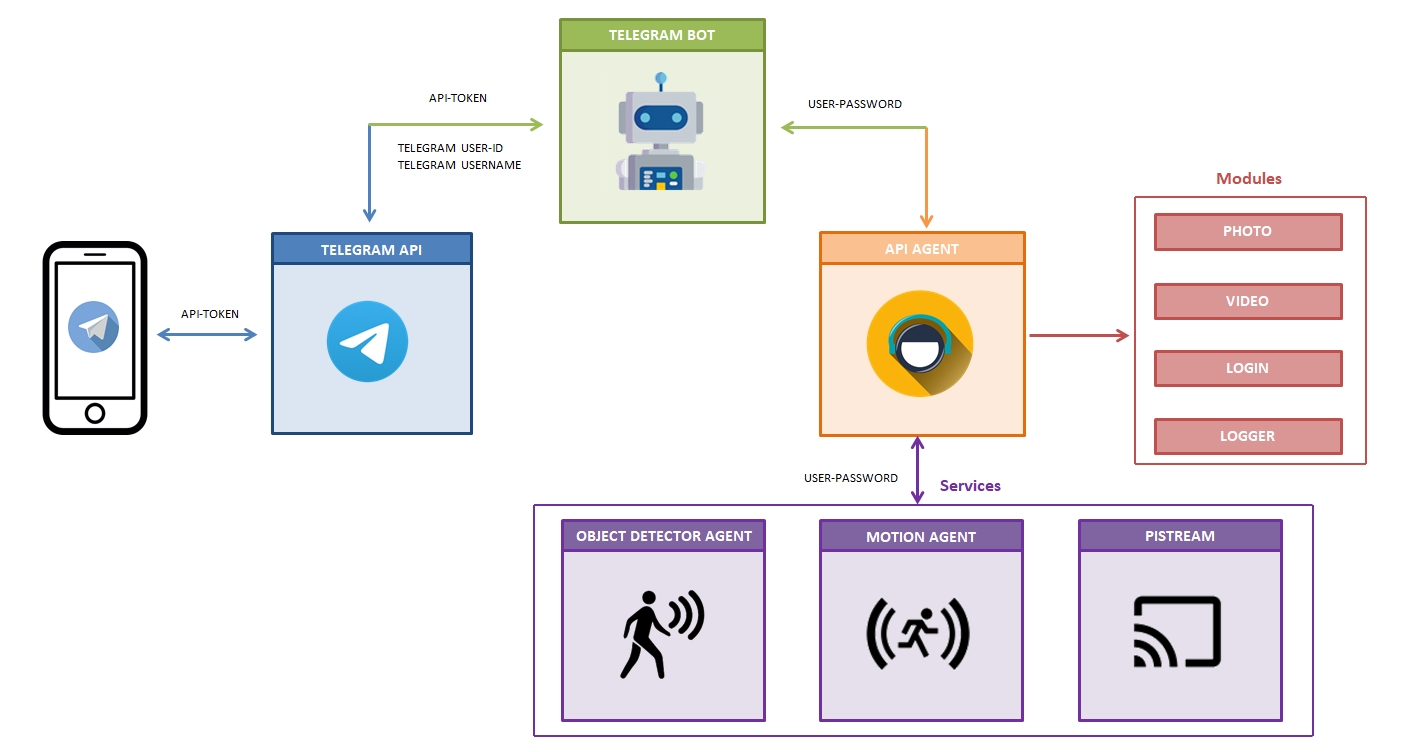
\includegraphics[scale=0.4]{images/23}
	\caption{Arquitectura de la aplicación}
	\label{img:arquitectura}
\end{figure}

En primer lugar tenemos los \textbf{módulos} de la aplicación (ver figura \ref{img:modulos}) que implementan un conjunto de funcionalidades para comunicarse con el módulo hardware de la cámara de la Raspberry PI, autenticación y logs.

\begin{figure}[h]
	\centering
	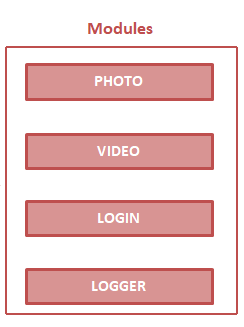
\includegraphics[scale=0.4]{images/24}
	\caption{Módulos de la aplicación}
	\label{img:modulos}
\end{figure}

A continuación tenemos el \textbf{API agent} (ver figura \ref{img:api}). Este es un servicio web que inicia la API que conecta con el resto de módulos de la aplicación.

\begin{figure}[h]
	\centering
	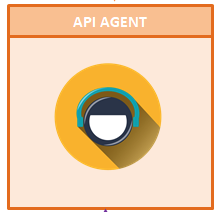
\includegraphics[scale=0.35]{images/25}
	\caption{API agent}
	\label{img:api}
\end{figure}

\newpage

Esta API importa y hace uso de los módulos de la aplicación. 

\begin{figure}[h]
	\centering
	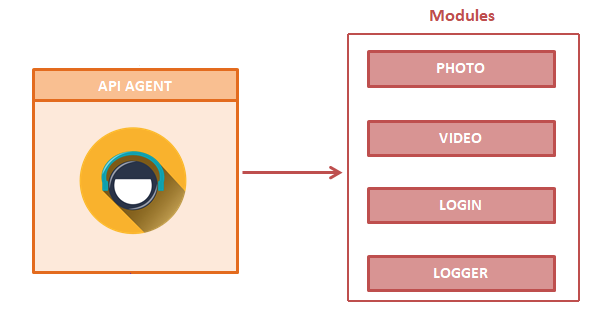
\includegraphics[scale=0.35]{images/27}
	\caption{Conexión entre la API y los módulos}
	\label{img:conexionapimodulos}
\end{figure}

Por otra parte, tenemos un conjunto de servicios que se inician de forma independiente y proporcionan las funcionalidades de detección de objetos en imágenes, detección de movimiento y servicio de streaming.

\begin{figure}[h]
	\centering
	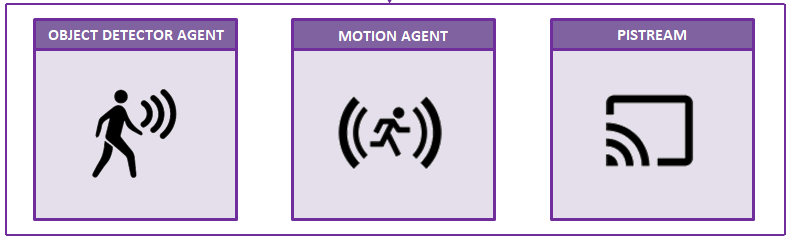
\includegraphics[scale=0.35]{images/26}
	\caption{Servicios de la aplicación}
	\label{img:serviciosaplicacion}
\end{figure}

La API está conectada con todo este conjunto de servicios y tiene la capacidad de poder gestionarlos.

\begin{figure}[h]
	\centering
	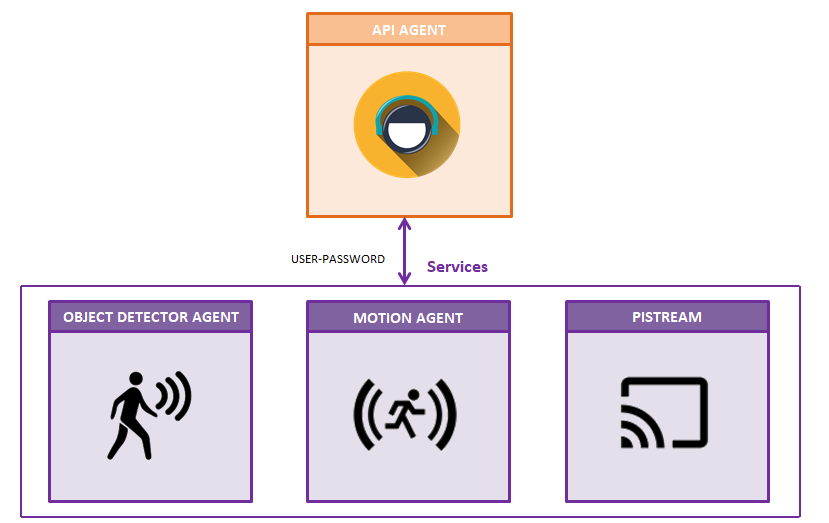
\includegraphics[scale=0.35]{images/28}
	\caption{Conexión entre los servicios y la API}
	\label{img:conexionserviciosapi}
\end{figure}

En la figura \ref{img:conexionmodulosserviciosapi} podemos ver, como quedan unidos todos estos componentes entre sí.

\newpage


\begin{figure}[h]
	\centering
	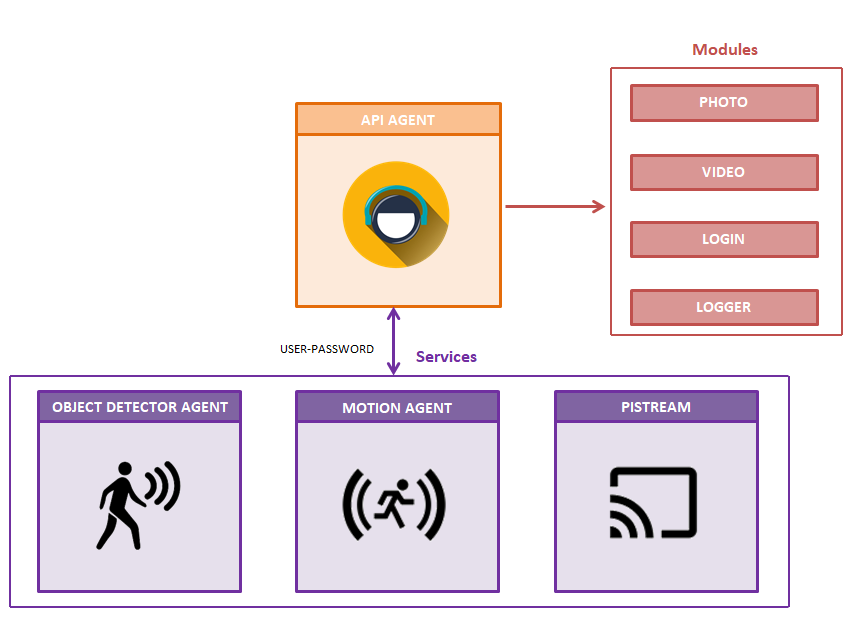
\includegraphics[scale=0.35]{images/35}
	\caption{Conexión de módulos y servicios con la API}
	\label{img:conexionmodulosserviciosapi}
\end{figure}

El siguiente componente es el \textbf{bot de Telegram}. Este bot es un proceso que se ejecuta junto a la API, cuyo objetivo es conectar la API de telegram con la API de la aplicación.

\begin{figure}[h]
	\centering
	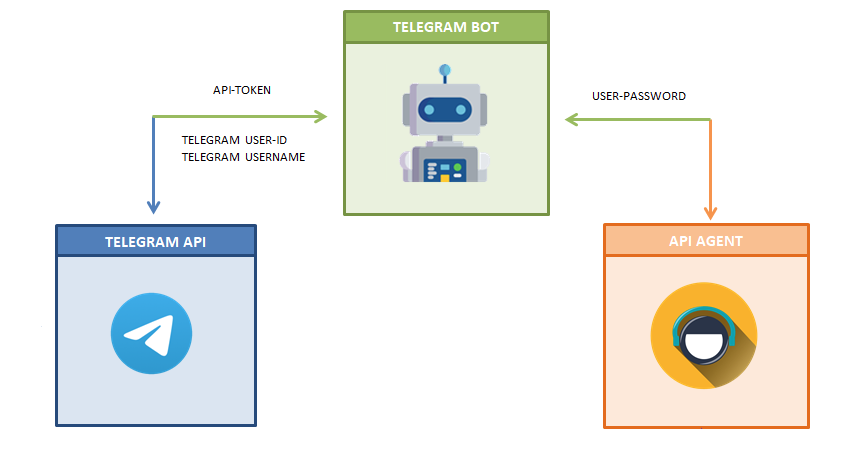
\includegraphics[scale=0.35]{images/34}
	\caption{Conexión entre el bot de telegram y la API}
	\label{img:conexionbotapitelegram}
\end{figure}

Finalmente, el usuario puede interactuar con la aplicación (\texttt{SIVIRA}), haciendo uso de la aplicación multiplataforma \texttt{Telegram}, usando el bot que se ha creado.

\begin{figure}[h]
	\centering
	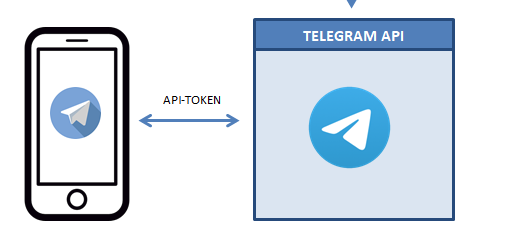
\includegraphics[scale=0.35]{images/33}
	\caption{Conexión entre el usuario y la aplicación}
	\label{img:usuariotelegram}
\end{figure}

\newpage

\subsection{Descripción de los componentes}

La aplicación (SIVIRA) desarrollada en este proyecto está compuesta por los siguientes componentes:

\subsubsection{Módulos}

Los módulos son un conjunto de funciones cuyo objetivo es encapsular funcionalidades que después serán utilizadas por el resto de componentes de la aplicación (ver figura \ref{img:modulos}). A continuación se realiza una descripción de cada uno de ellos.

\textbf{Logger}

Módulo cuyo objetivo es poder capturar y almacenar los logs de la aplicación en ficheros independientes para monitorizar el estado de la aplicación. Su implementación parte de una clase abstracta base, cuyo objetivo es definir las propiedades y métodos que tendrán todas las clases que implementarán los logs del sistema. 


PONER AQUÍ DIAGRAMA DE CLASES DE LOGS

\newpage

Por defecto, los logs son mostrados y almacenados de la siguiente forma:

\begin{itemize}
\item \textbf{Consola}: Corresponde a la salida \texttt{stdout}. Todo logs por encima de un nivel determinado de prioridad será mostrado por la salida de consola.

\item \textbf{Archivo de módulo}: Cada módulo y microservicio tendrán un fichero de log independiente para poder monitorizar su comportamiento a lo largo de su ejecución.

\item \textbf{Archivo de la aplicación}: La aplicación consta de un archivo de logs donde se almacenan todos los logs de módulos y microservicios de forma conjunta.

\item \textbf{Archivo de errores}: Todos los errores que surjan en cualquier módulo o microservicio es almacenado en este fichero para poder comprobar el estado de la aplicación.

\end{itemize}

Los niveles de logs que se han establecido son los siguientes:

\begin{itemize}

\item \textbf{DEBUG}: Nivel destinado a la depuración del código. Este nivel solo genera log en la salida por pantalla, y no se almacena en ningún fichero.

\item \textbf{INFO}: Nivel destinado a mostrar un mensaje informativo sobre alguna acción llevada a cabo. Estos logs son almacenados en el fichero de módulo correspondiente, en el fichero de logs de la aplicación y mostrados por pantalla.

\item \textbf{WARNING}: Nivel destinado a mostrar un mensajes de advertencia por posible mal uso de las llamadas a funciones, o simplemente porque algunas de ellas están '{deprecated}`. Estos logs son almacenados en el fichero de módulo correspondiente, en el fichero de logs de la aplicación y mostrados por pantalla.

\item \textbf{ERROR}: Nivel destinado a mostrar mensajes de error, que no son críticos para el sistema, y por lo tanto la aplicación sigue ejecutándose a pesar de producirse dichos error. Estos logs son almacenados en el fichero de módulo correspondiente, en el fichero de logs de la aplicación, en el fichero de errores de la aplicación.

\item \textbf{CRITICAL}: Nivel destinado a mostrar mensajes de error críticos que provocan el fallo de la aplicación. Estos logs son almacenados en el fichero de módulo correspondiente, en el fichero de logs de la aplicación, en el fichero de errores de la aplicación.

\end{itemize}



El formato por defecto de los logs es el siguiente:

\begin{itemize}
\item \textbf{Formato del archivo de errores}: \texttt{[Nivel:FechaHora:NombreArchivo:Función:Línea] Mensaje}. Por ejemplo:

\vspace{-1cm}

\begin{verbatim}

[ERROR:2019-08-15 13:10:11,597:logger.py:error:112x = set] Error while
trying to send an alert to Detector API agent with address 
http://192.168.1.100:11000.¿It is running?

\end{verbatim}


\vspace{-1cm}

\item \textbf{Formato del resto de logs}: \texttt{[Nivel:FechaHora] Mensaje}. Por ejemplo:

\vspace{-1.2cm}

\begin{verbatim}

[INFO:2019-08-13 18:35:03,278] A 5 seconds video is being 

\end{verbatim}

\end{itemize}

\vspace{-1.2cm}

Todos los ficheros de logs son almacenados en el directorio llamado \texttt{logs}. Dentro de dicho directorio, nos encontraremos los siguientes ficheros de logs:

\vspace{-0.4cm}

\begin{itemize}
\item \textbf{API\_agent.log}: Logs correspondientes a la API.
\item \textbf{detector\_object\_agent.log}: Logs correspondientes al agente detector de objetos.
\item \textbf{photo\_module.log}: Logs correspondientes al módulo de fotos.
\item \textbf{video\_module.log}: Logs correspondientes al módulo de vídeo.
\item \textbf{motion\_agent.log}: Logs correspondientes al agente detector de movimiento.
\item \textbf{security\_system\_PI\_app\_ERROR.log}: Logs correspondientes a los errores obtenidos por cualquier módulo o microservicio.
\item \textbf{security\_system\_PI\_app.log}: Logs correspondientes a los generados por módulos y microservicios a lo largo de su ejecución.
\item \textbf{telegram\_bot\_agent.log}: Logs correspondientes al bot de telegram.

\end{itemize}

La implementación de este módulo puede comprobarse en este \href{https://github.com/jmv74211/TFM_security_system_PI/blob/master/src/modules/logger.py}{enlace}.

\textbf{Photo} 

Módulo que implementa la clase \texttt{Photo} con la que se pretende administrar el recurso de la cámara de la Raspberry PI para capturar fotografías, además de establecer los diferentes parámetros de la cámara como resolución, rotación \ldots

Esta clase añade una capa de abstracción a la biblioteca \texttt{PiCamera} \cite{ref12}, para permitir conectarse con el recurso de la cámara de forma personalizada.

Las funcionalidades que aporta este módulo son las siguientes:

\vspace{-0.5cm}

\begin{itemize}
\item Capturar una fotografía.
\item Realizar una captura secuencial de fotografías en un intervalo de tiempo
\item Establecer la configuración de la cámara: Rotación, resolución, giro horizontal o giro vertical.

\end{itemize}

\vspace{-0.5cm}

La implementación de este módulo puede comprobarse en este \href{https://github.com/jmv74211/TFM_security_system_PI/blob/master/src/modules/photo.py}{enlace}.

\textbf{Video} 

Módulo que implementa la clase \texttt{Video} con la que se pretende administrar el recurso de la cámara de la Raspberry PI para realizar grabaciones de vídeo, además de establecer los diferentes parámetros de la cámara como resolución, rotación \ldots

Esta clase añade una capa de abstracción a la biblioteca \texttt{PiCamera} \cite{ref12}, para permitir conectarse con el recurso de la cámara de vídeo de forma personalizada.

Las funcionalidades que aporta este módulo son las siguientes:

\vspace{-0.5cm}

\begin{itemize}
\item Realizar una grabación de vídeo.
\item Conversión de formato de vídeo \texttt{.h264} a \texttt{.mp4} (compatible con telegram).
\item Establecer la configuración: Rotación, resolución, giro horizontal, giro vertical y mostrar hora y fecha durante la grabación de vídeo. .

\end{itemize}

\vspace{-0.5cm}

La implementación de este módulo puede comprobarse en este \href{https://github.com/jmv74211/TFM_security_system_PI/blob/master/src/modules/video.py}{enlace}.

\textbf{Authentication} 

Módulo implementado para realizar una autenticación en el sistema. Esta autenticación es solicitada por la API, ya que junto a la petición deberá de ir las credenciales de acceso que se han definido en la configuración de la aplicación.

Este módulo básicamente implementa una función para poder comprobar si la autenticación es correcta. Su implementación puede comprobarse en este \href{https://github.com/jmv74211/TFM_security_system_PI/blob/master/src/modules/authentication.py}{enlace}.

\subsubsection{Servicios}

Los servicios son procesos destinados a realizar alguna tarea en concreto y enviar una petición o respuesta con los resultados a la API. A continuación se realiza una descripción de cada uno de ellos.

\textbf{Motion agent}

Este servicio se encarga de controlar el sensor de movimiento y detectar cuando es activado para poder manejar dicho evento y enviar una alerta a la API. Las tareas realizadas por este servicio son las siguientes:

\vspace{-0.5cm}

\begin{itemize}
\item Controlar el estado del sensor.
\item Capturar fotos o vídeos en caso de detectar algún tipo de movimiento.
\item Enviar una petición para procesar la imagen capturada, con objetivo de poder detectar si hay alguna persona en ella.
\item Generar una alerta en la API en caso detectar a una persona en la foto.
\item Mover la foto generada por la alerta al directorio de \texttt{false\_positive} en caso de no detectar ninguna persona en la foto.

\end{itemize}

Para más información, en la sección X se detallará como funciona e interacciona este servicio con el resto de elementos.

La implementación de este servicio puede comprobarse en este \href{https://github.com/jmv74211/TFM_security_system_PI/blob/master/src/agents/motion_agent.py}{enlace}.

\textbf{Object detector agent}

Este servicio se encarga de procesar una foto y devolver una lista de objetos detectadas en dicha foto. Este servicio es usado por el \texttt{motion agent}, ya que cuando detecta movimiento (si la funcionalidad de detección de personas está activada), envía una petición a este servicio, y se le responde con la lista de objetos.

Esta funcionalidad ha sido implementada gracias al uso de la biblioteca de aprendizaje automático \texttt{Tensorflow} \cite{ref17}, ya que se ha utilizado para cargar el modelo preentrenado \texttt{ssdlite\_mobilenet\_v2\_coco} \cite{ref27} para poder predecir una lista de objetos que aparecen en una imagen.

El motivo por el cual se ha seleccionado ese modelo, es porque es el modelo más ligero, y el único viable para este proyecto en la Raspberry PI (debido a sus bajos recursos hardware). Antes de escoger este modelo, se hicieron pruebas con otros un poco más pesados y los resultados eran abrumadores. Utilizando otros modelos, se han obtenido una media de espera de más de 100 segundos para procesar la imagen (obviamente inviable).

Utilizar el modelo \texttt{ssdlite\_mobilenet\_v2\_coco} junto con una resolución de imagen media (1280x720) ha permitido obtener tiempos de procesamiento comprendidos entre unos 5 y 10 segundos, tiempo de espera que es aceptable.

El uso de este servicio es optativo, es decir, puede ser deshabilitado en las opciones o mediante la intefaz de usuario, y la aplicación puede funcionar normalmente. Es optativo por el hecho de su uso implica una serie de ventajas e inconvenientes que puede hacer pensar si realmente vale la pena utilizar este servicio o no.

Personalmente, yo recomendaría usar este servicio, ya que hay casos en los que se quiere controlar una zona y puede que haya demasiadas falsos positivos en las alertas por motivos como: animales domésticos, alta sensibilidad del sensor \ldots

A continuación se mencionan las posibles ventajas e inconvenientes de utilizar este servicio.

Ventajas

\begin{itemize}

\vspace{-0.5cm}

\item Evita posibles falsos positivos en las alertas generadas.
\item Puede aumentar el grado de eficacia del sistema de seguridad.
\end{itemize}

Desventajas

\vspace{-0.5cm}

\begin{itemize}
\item Añade sobrecarga de procesamiento en la Raspberry PI, calentamiento \ldots.
\item Añade latencia (5 a 10 segundos) en el momento de generar alertas, es decir, aumenta el tiempo desde que se produce un evento hasta que se envía la alerta.
\item Dado que el modelo de predicción es muy ligero, no es efectivo al 100\% y puede cometer algunos fallos.
\item Dificulta el proceso de instalación de la aplicación.
\end{itemize}

Por estos motivos, y porque la instalación de este agente puede resultar un poco tediosa (aunque todo está explicado en el repositorio del proyecto \cite{ref1}) se ha decidido entre realizar dos tipos de instalaciones de la aplicación, una en la que se utiliza otro servicio para filtrar eventos y reducir el número de falsos positivos en las alertas, y la otra en la que se prescinde totalmente de este servicio, y se genera una alerta tras la detección de cualquier movimiento.

La implementación de este servicio puede comprobarse en este \href{https://github.com/jmv74211/TFM_security_system_PI/blob/master/src/agents/object_detector_agent.py}{enlace}.





\newpage

\pagestyle{empty}

\begin{thebibliography}{99}

	\bibitem{ref1} Jonathan Martín Valera, TFM Security system PI github repository, disponible en \url{https://github.com/jmv74211/TFM_security_system_PI}

	\bibitem{ref2} Gus, 26 Jul 2019, Build a Raspberry Pi Security Camera Network,	disponible en \url{https://pimylifeup.com/raspberry-pi-security-camera/}
	
	\bibitem{ref3} ccrisan, 3 Sep 2019, A Video Surveillance OS For Single-board Computers ,	disponible en \url{https://github.com/ccrisan/motioneyeos}
	
	\bibitem{ref4} scavix, instructables.com, Raspberry Pi As Low-cost HD Surveillance Camera disponible en \url{https://www.instructables.com/id/Raspberry-Pi-as-low-cost-HD-surveillance-camera/}
	
	\bibitem{ref5} Motion-project, 19 Ago 2019, Camera video monitor, disponible en \url{https://github.com/Motion-Project/motion}
	
	\bibitem{ref6} Humberto Higinio, 14 Oct 2018, Sistema de Seguridad Raspberry Pi-Sensor de movimiento y cámara HD con envío de imágenes a correo, disponible en \url{https://www.youtube.com/watch?v=rK6uLwMRtIs}
	
	\bibitem{ref7} Google, DrawIO, diseño y diagramas de aplicaciones open source, disponible en \url{https://www.draw.io/}
	
	\bibitem{ref8} Visual paradigm, diseño de diagramas UML, disponible en \url{https://www.visual-paradigm.com/}
	
	\bibitem{ref9} Israel Alcázar, 03 Jun de 2014,  Introducción a Git y Github, disponible en \url{https://desarrolloweb.com/articulos/introduccion-git-github.html}
	
	\bibitem{ref10} Git, Sistema de control de versiones distribuido, multiplataforma y de código abierto, disponible en \url{https://git-scm.com/}
	
	\bibitem{ref11} Github, Servicio de alojamiento para el desarrollo de software utilizando Git , disponible en \url{https://git-scm.com/}
	
	\bibitem{ref12} PiCamera documentación, Interfaz de cámara Raspberry PI para python.
	
	\bibitem{ref13} pyTelegramBotAPI, Bibliotecas de funciones para la conexión con la API de telegram, disponible en \url{https://github.com/eternnoir/pyTelegramBotAPI}.
	
	\bibitem{ref14} Flask, framework para el despliegue ágil de aplicaciones sencillas, disponible en \url{https://flask.palletsprojects.com/en/1.1.x/}.
	
	\bibitem{ref15} Celery, Cola de tareas distribuidas, disponible en \url{http://www.celeryproject.org/}.
	
	\bibitem{ref16} RPi.GPIO, Biblioteca para controlar los pines GPIO de la Raspberry PI, disponible en \url{https://pypi.org/project/RPi.GPIO/}.
	
	\bibitem{ref17} Tensorflow, An end-to-end open source machine learning platform, disponible en \url{https://www.tensorflow.org/}.
	
	\bibitem{ref18} Requests, An end-to-end open source machine learning platform, disponible en \url{https://www.tensorflow.org/}.
	
	\bibitem{ref19} Latex-project, An introduction to LaTeX, disponible en \url{https://www.latex-project.org/about/}.

	\bibitem{ref20} TeX Live, 06 Jul de 2019, Introduction to TeX Live, disponible en \url{https://www.tug.org/texlive/}.
	
	\bibitem{ref21} TeXstudio.org, Welvome to TeXstudio, disponible en \url{https://www.texstudio.org/}.

	\bibitem{ref22} Jetbrains, Pycharm, The Python IDE
	for Professional Developers, disponible en \url{https://www.jetbrains.com/pycharm/}.
	
	\bibitem{ref23} RabbitMQ, Most widely deployed open source message broker, disponible en \url{https://www.rabbitmq.com/}.
	
	\bibitem{ref24} Telegram bot, Bots: An introduction for developers, disponible en \url{https://core.telegram.org/bots}.
	
	\bibitem{ref25} Olprod, 13 Nov 2018, Estilo de arquitectura de microservicios, disponible en \url{https://docs.microsoft.com/es-es/azure/architecture/guide/architecture-styles/microservices}.

	\bibitem{ref26} Chakray, 18 Jul 2018, DevOps: Arquitectura monolítica vs Microservicios, disponible en \url{https://www.chakray.com/es/devops-arquitectura-monolitica-vs-microservicios/}
	
	\bibitem{ref27} Tensorflow models ,Tensorflow detection model zoo, disponible en \url{https://github.com/tensorflow/models/blob/master/research/object_detection/g3doc/detection_model_zoo.md}
	
	\bibitem{ref28} MDN web docs, The WebSocket API (WebSockets), disponible en \url{https://developer.mozilla.org/en-US/docs/Web/API/WebSockets_API}
	
	\bibitem{ref29} waveform Pistreaming repository, A little demo of streaming the Pi's camera to web browsers, disponible en \url{https://github.com/waveform80/pistreaming}.
	
	\bibitem{ref30} Margaret Rouse, RESTful API, disponible en \url{https://searchapparchitecture.techtarget.com/definition/RESTful-API}
	
	\bibitem{ref31} Core telegram , Telegram APIs and Bot API, disponible en \url{https://core.telegram.org/}
	
	\bibitem{ref32} eternnoir pyTelegramBotAPI, A simple, but extensible Python implementation for the Telegram Bot API, disponible en \url{https://github.com/eternnoir/pyTelegramBotAPI}
	
	
	\bibitem{refx1} Core telegram, New Inline Keyboards, disponible en \url{https://core.telegram.org/bots/2-0-intro}
	
\end{thebibliography}

\end{document}



% ###################	FIN DEL DOCUMENTO ###################